% TODO: 
% query optimization 2 статья лежит, добавить
% 1) слушатели не знали что такое представление, надо расписать
% 2) сделать ``анимацию'' в алгоритме, с примером на таблице?
% 3) часть про три оптимизатора бедна, надо больше рассказать











%%%%%%%%%%%%%%%%%%%%%%%%%%%%%%%%%%%%%%%%%
% Beamer Presentation
% LaTeX Template
% Version 1.0 (10/11/12)
%
% This template has been downloaded from:
% http://www.LaTeXTemplates.com
%
% License:
% CC BY-NC-SA 3.0 (http://creativecommons.org/licenses/by-nc-sa/3.0/)
%
%%%%%%%%%%%%%%%%%%%%%%%%%%%%%%%%%%%%%%%%%

%----------------------------------------------------------------------------------------
%	PACKAGES AND THEMES
%----------------------------------------------------------------------------------------

\documentclass{beamer}

\mode<presentation> {

% The Beamer class comes with a number of default slide themes
% which change the colors and layouts of slides. Below this is a list
% of all the themes, uncomment each in turn to see what they look like.

%\usetheme{default}
%\usetheme{AnnArbor}
%\usetheme{Antibes}
%\usetheme{Bergen}
%\usetheme{Berkeley}
%\usetheme{Berlin}
%\usetheme{Boadilla}
%\usetheme{CambridgeUS}
%\usetheme{Copenhagen}
%\usetheme{Darmstadt}
%\usetheme{Dresden}
%\usetheme{Frankfurt}
%\usetheme{Goettingen}
%\usetheme{Hannover}
%\usetheme{Ilmenau}
%\usetheme{JuanLesPins}
%\usetheme{Luebeck}
\usetheme{Madrid}
%\usetheme{Malmoe}
%\usetheme{Marburg}
%\usetheme{Montpellier}
%\usetheme{PaloAlto}
%\usetheme{Pittsburgh}
%\usetheme{Rochester}
%\usetheme{Singapore}
%\usetheme{Szeged}
%\usetheme{Warsaw}

% As well as themes, the Beamer class has a number of color themes
% for any slide theme. Uncomment each of these in turn to see how it
% changes the colors of your current slide theme.

%\usecolortheme{albatross}
%\usecolortheme{beaver}
%\usecolortheme{beetle}
%\usecolortheme{crane}
%\usecolortheme{dolphin}
%\usecolortheme{dove}
%\usecolortheme{fly}
%\usecolortheme{lily}
%\usecolortheme{orchid}
%\usecolortheme{rose}
%\usecolortheme{seagull}
%\usecolortheme{seahorse}
%\usecolortheme{whale}
%\usecolortheme{wolverine}

%\setbeamertemplate{footline} % To remove the footer line in all slides uncomment this line
%\setbeamertemplate{footline}[page number] % To replace the footer line in all slides with a simple slide count uncomment this line

%\setbeamertemplate{navigation symbols}{} % To remove the navigation symbols from the bottom of all slides uncomment this line
}

\usepackage[utf8]{inputenc}
\usepackage[russian]{babel}
\usepackage{cmap}


\usepackage{verbatim}
\usepackage{fancybox}
\usepackage{ulem}
\usepackage{tikz}
\usetikzlibrary{positioning}
\usepackage{scalefnt}
\usetikzlibrary{arrows,shapes,positioning,shadows,trees,calc,backgrounds,fit,positioning}

\usepackage{graphicx} % Allows including images
\usepackage{booktabs} % Allows the use of \toprule, \midrule and \bottomrule in tables
\usepackage{textcomp}
\usepackage{listings}
\usepackage{color}
\usepackage{xcolor}
\usepackage{changepage}
\usepackage{longtable}

\definecolor{mygreen}{rgb}{0,0.6,0}
\definecolor{mygray}{rgb}{0.5,0.5,0.5}
\definecolor{mymauve}{rgb}{0.58,0,0.82}

\lstset{ %
  backgroundcolor=\color{white},   % choose the background color; you must add \usepackage{color} or \usepackage{xcolor}
  basicstyle=\footnotesize,        % the size of the fonts that are used for the code
  breakatwhitespace=false,         % sets if automatic breaks should only happen at whitespace
  breaklines=true,                 % sets automatic line breaking
  captionpos=b,                    % sets the caption-position to bottom
  commentstyle=\color{mygreen},    % comment style
  deletekeywords={...},            % if you want to delete keywords from the given language
  escapeinside={\%*}{*)},          % if you want to add LaTeX within your code
  extendedchars=true,              % lets you use non-ASCII characters; for 8-bits encodings only, does not work with UTF-8
  frame=single,                    % adds a frame around the code
  keepspaces=true,                 % keeps spaces in text, useful for keeping indentation of code (possibly needs columns=flexible)
  keywordstyle=\color{blue},       % keyword style
  language=Octave,                 % the language of the code
  morekeywords={*,...},            % if you want to add more keywords to the set
  numbers=left,                    % where to put the line-numbers; possible values are (none, left, right)
  numbersep=5pt,                   % how far the line-numbers are from the code
  numberstyle=\tiny\color{mygray}, % the style that is used for the line-numbers
  rulecolor=\color{black},         % if not set, the frame-color may be changed on line-breaks within not-black text (e.g. comments (green here))
  showspaces=false,                % show spaces everywhere adding particular underscores; it overrides 'showstringspaces'
  showstringspaces=false,          % underline spaces within strings only
  showtabs=true,                  % show tabs within strings adding particular underscores
  stepnumber=1,                    % the step between two line-numbers. If it's 1, each line will be numbered
  stringstyle=\color{mymauve},     % string literal style
  tabsize=4,                       % sets default tabsize to 2 spaces
  %title=\lstname                   % show the filename of files included with \lstinputlisting; also try caption instead of title
}

\graphicspath{{./figures/}}

%----------------------------------------------------------------------------------------
%	TITLE PAGE
%----------------------------------------------------------------------------------------

\title[Обработка и исполнение запросов: лекция 2]{Обработка и исполнение запросов в СУБД (Лекция 2) \\~\\ Классические системы: оптимизация запросов в реляционных СУБД\\~\\ v6} % The short title appears at the bottom of every slide, the full title is only on the title page

\author{Георгий Чернышев} % Your name
\institute[ВШЭ] % Your institution as it will appear on the bottom of every slide, may be shorthand to save space
{
Высшая Школа Экономики \\ % Your institution for the title page
\medskip
\textit{chernishev@gmail.com} % Your email address
}
%\date{\today} % Date, can be changed to a custom date

\date{9 сентября 2020 г.}

\begin{document}

\begin{frame}
\titlepage % Print the title page as the first slide
\end{frame}

\begin{comment}
\begin{frame}
\frametitle{Overview} % Table of contents slide, comment this block out to remove it
\tableofcontents % Throughout your presentation, if you choose to use \section{} and \subsection{} commands, these will automatically be printed on this slide as an overview of your presentation
\end{frame}
\end{comment}

\begin{frame}
\frametitle{Основные компоненты классической реляционной СУБД}

\begin{figure}[htb]
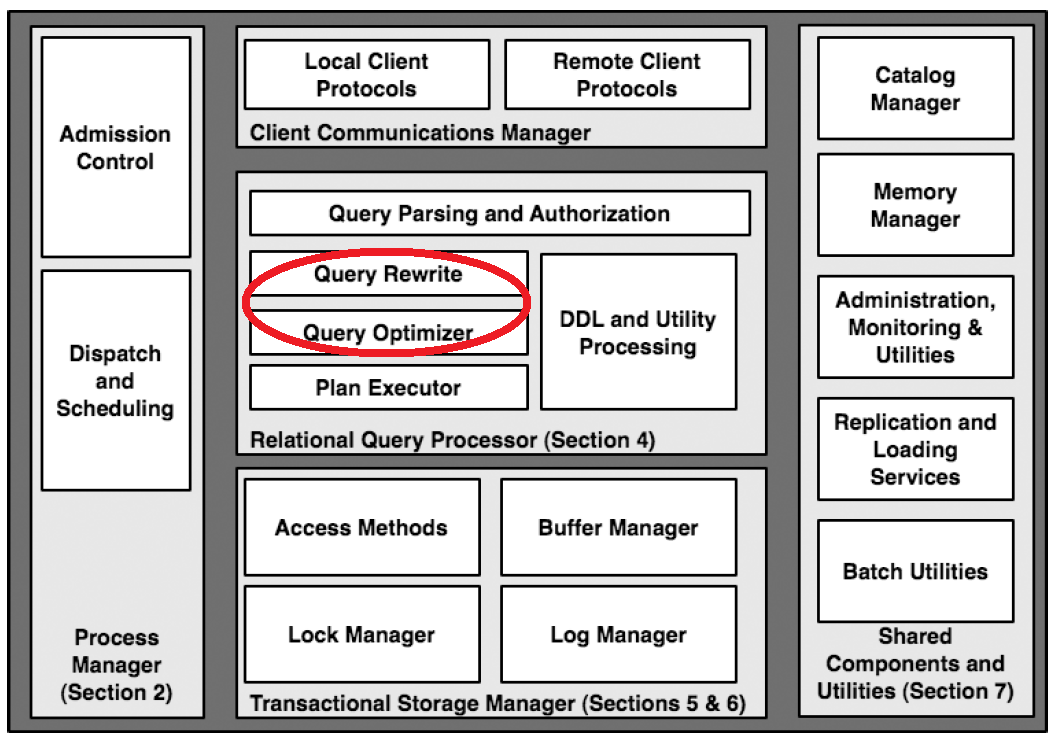
\includegraphics[width=\textwidth,height=0.75\textheight,keepaspectratio]{overall-schema.png} 
\footnote{\tiny{Изображение взято из \cite{Hellerstein2007}}}
\end{figure}
\end{frame}

\begin{frame}
\frametitle{Напоминание: стадии обработки запроса}
\begin{itemize}
  \setlength\itemsep{1em}
  \item Разбор и авторизация;
  \item Перезапись запроса;
  \item Оптимизация запроса;
  \item Выполнение запроса.
\end{itemize}
\end{frame}

\begin{frame}[allowframebreaks]
\frametitle{Перезапись запроса}
Некоторые преобразования не меняющие семантики запроса, но упрощающие/удешевляющие выполнение. 
\\~\\
Идея: пользуемся только запросом и каталогом, на сами данные не смотрим.
\\~\\
Раньше это всегда была отдельная фаза, сейчас не всегда, иногда её вкладывают в оптимизатор.

\end{frame}

\begin{frame}[allowframebreaks]
\frametitle{Основные типы преобразований}
Некоторые преобразования не меняющие семантики запроса, но упрощающие/удешевляющие выполнение. Основные типы \cite{Hellerstein2007}:
\begin{itemize}
  \item Перезапись представлений (исторически~--- основное предназначение):
  		раскрыть представление, найти исходные таблицы, подставить ссылки на них, перенести предикаты из представления:
  		
CREATE VIEW [Brazil Customers] AS SELECT CustomerName, ContactName, Status FROM Customers WHERE Country = 'Brazil';\\
...\\
SELECT * FROM [Brazil Customers] WHERE Status = 1;\\
$\Longrightarrow$\\
SELECT CustomerName, ContactName, Status FROM Customers WHERE Country = 'Brazil' AND Status = 1; 	
  \item Вычисление константных выражений:\\
SELECT 2 + 2 AS result, * FROM R WHERE R.x < 10+2+R.y\\
$\Longrightarrow$\\
SELECT 4 AS result, * FROM R WHERE R.x < 12+R.y
  %\framebreak
  \item Перезапись предикатов из WHERE:
  \begin{itemize}
    \setlength\itemsep{1em}
    \item упрощение для использования подходящего access method:\\
    NOT Emp.Salary > 1000000\\
    $\Longrightarrow$\\
    Emp.Salary <= 1000000
    \item упрощение для поиска конфликтующих условий:\\
    Emp.salary < 75000 AND Emp.salary > 1000000\\
    $\Longrightarrow$\\
    $\{\}$
    \item распространение предикатов по транзитивности:\\
    R.x < 10 AND R.x = S.y\\
    $\Longrightarrow$\\
    AND S.y < 10
  \end{itemize}
  %\framebreak
  \item Семантическая оптимизация:
  \begin{itemize}
  \setlength\itemsep{1em}
    \item Например, учет ограничений целостности для redundant join elimination:\\   
    SELECT Emp.name, Emp.salary FROM Emp, Dept WHERE Emp.deptno = Dept.dno\\
    Если если есть FK Emp.deptno к Dept, то...
    $\Longrightarrow$ \alert{не надо соединять!}
    Классический способ решения проблемы поддержки ``широких'' таблиц (например, в Siebel).
  \end{itemize}
  \framebreak
  
  В случае вложенных запросов оптимизатор работает с блоками SELECT-FROM-WHERE, поодиночке. Почему? Чтобы \underline{уменьшить сложность работы}!
  
  \item Что делают при работе с блоками на фазе рерайта:
  \begin{itemize}
    \setlength\itemsep{1em}
    \item Подготовка блока к оптимизации~--- нормализация запроса (получение канонической формы, как вариант);
    \item Уплощение запроса (раскрытие подзапросов): иногда\footnote{https://db.apache.org/derby/docs/10.6/tuning/ctuntransform36368.html} подзапрос можно переписать в соединение;
    \item Межблочный перенос предикатов с использование транзитивности\footnote{упражнение: придумать самому};
    \item Распараллеливание кореллированных подзапросов\footnote{https://en.wikipedia.org/wiki/Correlated\_subquery}.
  \end{itemize}
\end{itemize}

\end{frame}



\begin{comment}

\begin{frame}[allowframebreaks]
\frametitle{QGM: пример}

\begin{figure}[htb]
\includegraphics[width=\textwidth,height=0.5\textheight,keepaspectratio]{qgm1.png} 
\footnote{\tiny{Изображение взято из \cite{Haas1989}}}
\end{figure}


\begin{figure}[htb]
\includegraphics[width=\textwidth,height=0.75\textheight,keepaspectratio]{qgm2.png} 
\footnote{\tiny{Изображение взято из \cite{Haas1989}}}
\end{figure}
\end{frame}



\begin{frame}
\frametitle{Оптимизация запроса II}

\begin{block}{Цель:}
для данного запроса выбрать лучшую стратегию выполнения при условии заданных ресурсных ограничений \cite{Neumann2009}.
\end{block}

\begin{itemize}
  \item Volcano, Cascades \cite{Graefe1993}, \cite{Graefe1995}: 
  \begin{itemize}
    \item Кеширующая сборка дерева сверху вниз;
    \item \alert{Трансформационный оптимизатор}.
  \end{itemize}
  
\end{itemize}
\end{frame}

\end{comment}

\begin{frame}[allowframebreaks]
\frametitle{Оптимизация в первом приближении:}

\begin{figure}[htb]
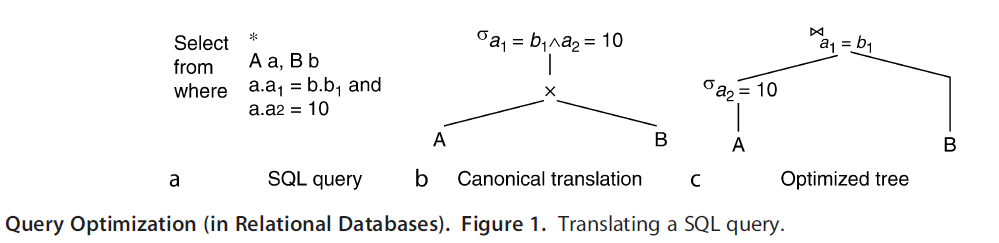
\includegraphics[width=\textwidth,height=0.75\textheight,keepaspectratio]{optimization.png} 
\footnote{\tiny{Изображение взято из \cite{Neumann2009}}}
\end{figure}


Порядок:
\begin{itemize}
  \item Текст запроса;
  \item Каноническое представление;
  \item Оптимизированный план.
\end{itemize}

\end{frame}

\begin{frame}[allowframebreaks]
\frametitle{Трансформационный оптимизатор}

Алгебраические эквивалентности:
$$ A \bowtie B \equiv  B \bowtie A$$

$$ A \bowtie (B \bowtie C)\equiv (A \bowtie B) \bowtie C  $$

База для построения \alert{трансформационных} оптимизаторов:
\begin{itemize}
  \setlength\itemsep{1em}
  \item Просто (проще) строить;
  \item Сложно сделать эффективный обход пространства планов $\Rightarrow$ большинство из них это эвристические оптимизаторы.
\end{itemize}

\end{frame}

\begin{frame}[allowframebreaks]
\frametitle{Конструктивный оптимизатор}

Альтернатива:

\begin{itemize}
  \setlength\itemsep{1em}
  \item Не применяет эквивалентности как основное средство перебора пространства планов;
  \item Cтроит план из кусочков, чаще всего снизу вверх;
  \item Может эффективно обходить пространство планов;
  \item Этим способом сложные эквивалентности трудно находить и применять, поэтому трансформационный шаг нужен:
  \begin{itemize}
    \item вынесен на rewrite или пост-оптимизационную фазу.
  \end{itemize}
  
\end{itemize}
  Как строить план из кусочков? Оценивая стоимости.

\end{frame}
%%

\begin{frame}
\frametitle{Конструктивный оптимизатор II: стоимости}

\begin{itemize}
  \item Самая простая идея: количество обработанных записей
  \begin{itemize}
    \item алгебра (реляционные операции) + статистика + селективность;
    \item неточна, на практике работает плохо.
  \end{itemize} 
  \item Сложные модели:
  \begin{itemize}
    \item вычисляем ожидаемое время выполнения;
    \item учитываются шаблоны доступа к диску, стоимости вычисления ``дорогих'' предикатов и т.д.;
    \item обычно стоимостная функция это линейная комбинация стоимостей I/O и CPU;
    \item \alert{в алгебре таких параметров нет}.
  \end{itemize} 
  
\end{itemize}

Селективность предиката это вероятность того, что запись ему будет удовлетворять. Высокоселективный предикат это предикат возвращающий мало записей из таблицы.

\end{frame}

\begin{frame}[allowframebreaks]
\frametitle{Логическая и физическая алгебра}


\begin{itemize}
  \setlength\itemsep{1em}
  \item Логическая алгебра: 
  \begin{itemize}
    \setlength\itemsep{1em}
    \item концепции операторов, известных движку базы данных;
    \item более абстрактна, позволяет трансформации;
  \end{itemize}
  
  \item Физическая алгебра:
  \begin{itemize}
    \setlength\itemsep{1em}
    \item реализация этих концепций;
    \item физическая алгебра ``знает'' параметры;
    \item в этой алгебре представлен результат работы оптимизатора.
  \end{itemize} 
\end{itemize}

Пример: оператор внутреннего соединения~--- логическая алгебра; реализация оператора внутреннего соединения методом nested loop~--- физическая алгебра.

\end{frame}

\begin{frame}[allowframebreaks]
	\frametitle{Оптимизация запроса}
	
	\begin{block}{Цель:}
		для данного запроса выбрать лучшую стратегию выполнения при условии заданных ресурсных ограничений \cite{Neumann2009}.
	\end{block}
	
	\begin{itemize}
		\item System R \cite{Selinger1979}: 
		\begin{itemize}
			\item Первый оптимизатор;
			\item Динамическое программирование для выбора порядка соединений;
			\item Придумали ``interesting orders'', учет отсортированности данных;
		\end{itemize}
		\item Оптимизатор Starburst \cite{Haas1989}:
		\begin{itemize}
			\item Использует правила для комбинирования физических операторов;
			\item Подобна System R, сборка снизу вверх;
			\item Новое внутреннее представление (Query Graph Model).
		\end{itemize}
		\item Volcano, Cascades \cite{Graefe1993}, \cite{Graefe1995}: 
		\begin{itemize}
			\item Кеширующая сборка дерева сверху вниз;
			\item Трансформационный оптимизатор.
		\end{itemize} 
	\end{itemize}
	
\end{frame}

\begin{frame}
\frametitle{Дерево операторов I}

Рассматриваем простой класс запросов: SPJ без подзапросов\\
Select-Project-Join = SELECT ... FROM ... WHERE ...
\begin{itemize}
  \setlength\itemsep{1em}
  \item полностью описывается 
  \begin{itemize}
    \item выборка ($\sigma$) 
    \item соединение/прямое произведение ($\bowtie/\times$)
    \item проекция ($ \prod$)
  \end{itemize}
  \item задача нахождения оптимального плана для него $NP$-трудна!
  \item если оставить только соединения и прямые произведения то...
  \begin{itemize}
    \item и эта задача $NP$-трудна;
    \item = задаче поиска оптимального бинарного дерева с $n$ листьями;
    \item а количество таких деревьев = число Каталана: $\mathcal{C}(n-1)$;
    \item которое растет как $\theta (\frac{4^n}{n^{3/2}})$.
  \end{itemize}

\end{itemize}

\end{frame}

\begin{frame}
\frametitle{Дерево операторов II}

\begin{figure}[htb]
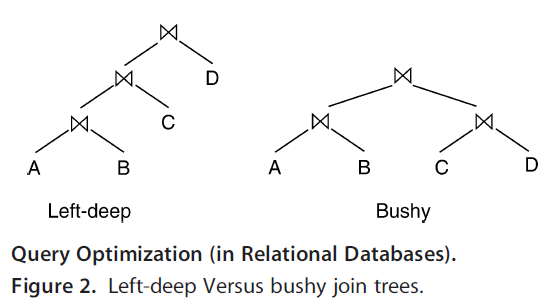
\includegraphics[width=\textwidth,height=0.3\textheight,keepaspectratio]{trees.png} 
\footnote{\tiny{Изображение взято из \cite{Neumann2009}}}
\end{figure}


\begin{itemize}
  \item Надо упрощать задачу дальше: линейные деревья и лево-линейные деревья;
  \begin{itemize}
    \item проще выполнять;
    \item их ``всего'' $n!$, проще перебирать при поиске;
    \item оптимального может и не оказаться: кустистых больше~--- $n!\mathcal{C}(n-1)$
    \item ... да скорее всего не окажется + кустистые хорошо параллелятся;
  \end{itemize}  
\end{itemize}

\end{frame}

\begin{frame}
\frametitle{Дерево операторов III}

\scriptsize  
``Объединять'' два отношения можно с помощью $\bowtie$ или же $\times$:

\begin{itemize}
	\item Чаще всего $\bowtie$ эффективнее.
	\item Однако бывают случаи когда лучше сделать $\times$ (упражнение).
\end{itemize}

Когда можно делать $\bowtie$?

\begin{figure}[htb]
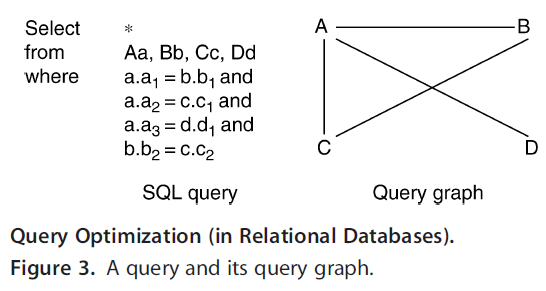
\includegraphics[width=\textwidth,height=0.3\textheight,keepaspectratio]{cross.png} 
\footnote{\tiny{Изображение взято из \cite{Neumann2009}}}
\end{figure}

Не всегда можно соединять без прямых произведений (e.g. B, C, D). Две крайности:

\begin{itemize}
  \item Линейный граф, тогда $O(N^3)$;
  \item Полный граф, тогда опять же $NP$-hard.
\end{itemize}

Обычно, реальный случай где-то посередине.

\normalsize

\end{frame}

\begin{frame}
\frametitle{Промежуточный итог}

Стандартный подход~--- строим оптимизационный алгоритм исходя из следующих положений:

\begin{itemize}
  \setlength\itemsep{1em}
  \item Оптимизируем только порядок соединений;
  \item Проекции и агрегации добавляем сверху, снизу жадно выборки;
  \item Используем граф соединений для проверки возможности соединения;
  \item Строим \alert{лево-линейные деревья}, правая сторона соединения содержит только одного ребенка.
\end{itemize}

\end{frame}


\begin{frame}
\frametitle{Алгоритм}

\begin{figure}[htb]
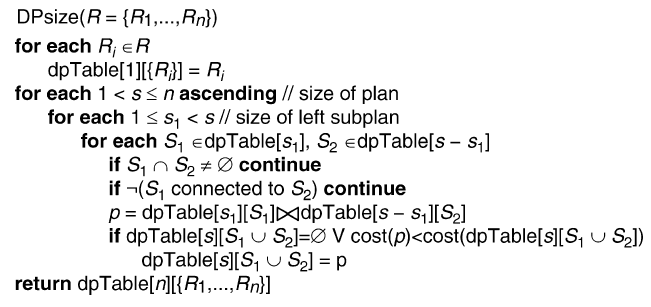
\includegraphics[width=\textwidth,height=0.59\textheight,keepaspectratio]{algorithm.png} 
\footnote{\tiny{Изображение взято из \cite{Neumann2009}}}
\end{figure}

Улучшенный алгоритм из \cite{Selinger1979}, в нем мы строим \alert{кустистые деревья}!

\end{frame}

\begin{frame}
	\frametitle{Пример}

Демонстрация.
\end{frame}

\begin{frame}
\frametitle{Пояснения по алгоритму}

\begin{itemize}
  \item Динамическое программирование, даны $n$ отношений $R_1, ..., R_n$;
  \item Строим таблицу где будут стоимости, инициализируем стоимостью скана;
  \item $s$~--- строим план по возрастанию, $s_1$~--- левый план;
  \item Проходимся по парам $S_1$, $S_2$ (уже посчитанный промежуточный результат);
  \item Если пересекаются то нельзя соединить;
  \item Если нет предиката то тоже пропускаем, прямых произведений не создаем;
  \item Иначе, если выгодно соединять~--- соединяем.
\end{itemize}

\end{frame}

\begin{frame}
\frametitle{Замечания по алгоритму}
Алгоритм упрощенный:
\begin{itemize}
  \item Нет выборок, проекций, но можно добавить в строки 2 и 8 (неоптимально);
  \item Нет выбора физического оператора соединения, добавляем в 8--10 строку;
  \item Sort-Merge ведет себя очень по-разному, надо хранить interesting orders;
  \begin{itemize}
    \item это, в свою очередь, ведет к структуре physical properties~--- характеристика плана, вляющая на исполнение (в будущем), но не на логическую эквивалентность;
    \item цель: пытаемся сохранить упорядоченность для будущих итераций алгоритма;
    \item концепция доминирования: план X доминирует план Y, если имеет те же самые physical properties и его стоимость меньше;
    \item в dpTable находятся наборы планов, в которых нет доминирующих пар;
  \end{itemize}
\end{itemize}

\end{frame}

\begin{frame}
	\frametitle{О более production-ready алгоритмах и распараллеливании}

Еще информации про несовсем ``игрушечные'' алгоритмы:

\scriptsize

Meister A., Saake G. (2017) Cost-Function Complexity Matters: When Does Parallel Dynamic Programming Pay Off for Join-Order Optimization. ADBIS 2017.

\normalsize

О распараллеливании (изображение оттуда же):

\begin{figure}[htb]
	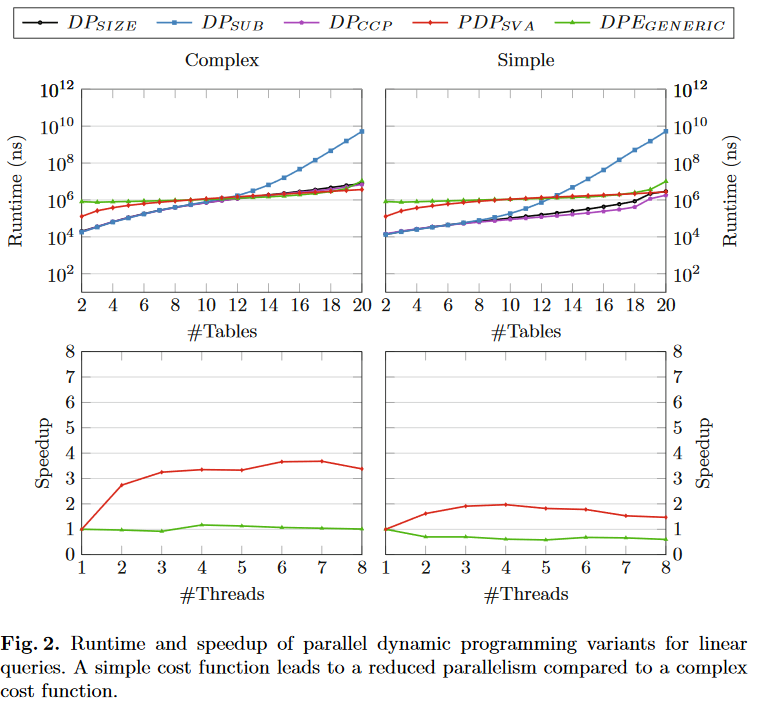
\includegraphics[width=\textwidth,height=0.630\textheight,keepaspectratio]{parallel-dp-enumeration.png}
\end{figure}

\end{frame}


\begin{frame}
\frametitle{Замечания по оптимизации сложных запросов}

\begin{itemize}
  \item Говоря соединение выше имелось ввиду внутреннее соединение, в случае внешних\footnote{\url{http://www.datamartist.com/sql-inner-join-left-outer-join-full-outer-join-examples-with-syntax-for-sql-server}} всё будет сложнее~--- оно не коммутативно и не ассоциативно;
  \item Агрегацию можно бездумно проталкивать вниз, под соединения, если выше находятся соединения 1 к 1 (в некоторых случаях можно делать пре-аггрегацию, не смотря на тип соединения);
  \item Бывают вложенные запросы:\\ SELECT ... WHERE X IN (SELECT ...);
  \begin{itemize}
    \item Можно бить на блоки и обрабатывать их отдельно, но часто невыгодно;
    \item Вместо этого: стараться пропихнуть внешние предикаты внутрь или попытаться уплощить запрос.
  \end{itemize}
\end{itemize}

\end{frame}

\begin{frame}[allowframebreaks]
\frametitle{Как обстоят дела с оптимизацией запросов в индустриальном мире}

\begin{columns}
	\begin{column}{0.48\textwidth}	
		\begin{itemize}
			\item ученые в современных статьях могут делать до 500 соединений однако...
			\item ...если много таблиц (6--15+), индустриальные системы часто переходят на эвристические методы...
			\item ...и виноваты в этом методы сбора статистики!
			\item появление новых моделей и систем привел к всплеску интереса к тематике, очень много работ на топовых БД-конференциях от компаний
		\end{itemize}
		
	\end{column}
	\begin{column}{0.48\textwidth}
		\begin{figure}[htb]
			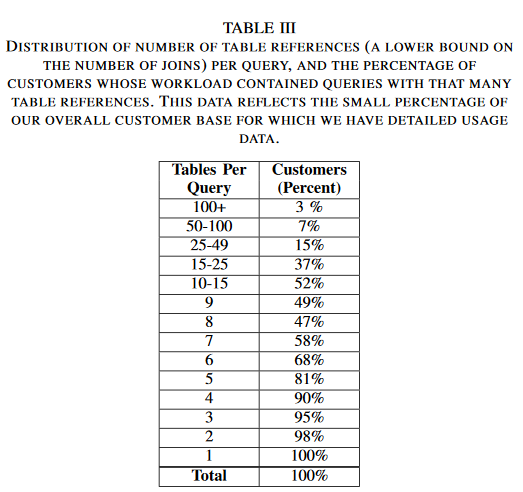
\includegraphics[width=\textwidth,height=0.930\textheight,keepaspectratio]{tablenum.png}\footnote{Изображение взято из \cite{Vertica}}
		\end{figure}			
	\end{column}
\end{columns}

Теперь про конкретные индустриальные системы:

\scriptsize



\begin{table}

\begin{longtable}{|p{2cm}|c|c|p{7.2cm}|}
	\hline
	СУБД & год  & тип  & Оптимизатор \\
	\hline
	
	PostgreSQL & 1996 & D & Стоимостной оптимизатор, переупорядочивает соединения, использует генетический алгоритм для обхода\footnote{\url{https://postgrespro.com/docs/postgresql/11/geqo-intro2.html}}\\
	
	MariaDB & 1995 & D & До 2012 года не использовала статистику вообще\footnote{\url{https://mariadb.com/kb/en/differences-between-the-mysql-and-mariadb-query-optimizer/}}, работали на эвристиках. Сейчас умеют переупорядочивать соединения\footnote{\url{https://www.oreilly.com/library/view/high-performance-mysql/9780596101718/ch04.html}}, еще список\footnote{\url{https://mariadb.com/kb/en/query-optimizations/}} чего умеют.\\
	
	SQLite & 2000 & M & Оптимизируют (стоимостно) index-based nested-loop joins\footnote{\url{https://www.sqlite.org/queryplanner-ng.html}} (порядок и используемый индекс). В прошлой версии использовалась эвристика ``ближайший сосед'' на графе соединений, теперь ``N ближайших''. Другие интересные оптимизации\footnote{\url{https://www.sqlite.org/optoverview.html}}.\\
	

	Sybase Adaptive Server Enterprise & 1987 & D & Стоимостной оптимизатор	\footnote{\url{http://infocenter.sybase.com/help/index.jsp?topic=/com.sybase.infocenter.dc00743.1502/html/queryprocessing/BHCDBECI.htm}}: типы, порядок соединений. Есть выделенная фаза рерайта: трансформации предикатов~--- транзитивное замыкание, схлопывание и т.д.\\

	\hline
	\hline
	
	Vertica & 2005 & D & Стоимостной оптимизатор для Data Warehouse системы: есть рерайтер, выбор порядка соединений, выбор проекций для работы (система колоночная, с репликацией)\footnote{ The Vertica Query Optimizer: The case for specialized query optimizers}.\\
	
	
	Snowflake & 2012 & D & Облачная DW система, нацелена на убирание ``tuning knobs'' (нет индексов, partition keys, только кластеризация и автотюнинг ~--- 11 лекция)\footnote{https://www.snowflake.com/blog/automatic-query-optimization-no-tuning/}.\\
	
	Microsoft SQL server PDW & 2012? & D & Классический двухшаговый\footnote{Query optimization in microsoft SQL server PDW} (ждите 5 пятой лекции) распределенный стоимостной оптимизатор. Это не база данных, а еще и железка!\\
	
	MemSQL & 2013 & D/M & Классический стоимостной оптимизатор с рерайтером (есть интересные!), есть подробности про распределенную оптимизацию\footnote{The MemSQL Query Optimizer: A modern optimizer for real-time analytics in a distributed database}, e.g. стоимости решафлинга.\\
	
	GreenPlum & 2005 & D & Не оптимизатор, а фреймворк для создания оптимизаторов\footnote{Orca: a modular query optimizer architecture for big data}. Полезно посмотреть для ``суммаризации'' знаний по предмету.\\

	
	
	
	
	
	\hline
\end{longtable}

\end{table}	

\end{frame}

\begin{frame}[allowframebreaks]
\frametitle{Ссылки}
\footnotesize{
\begin{thebibliography}{99}

%\bibitem[Garcia-Molina et al., 2004] {Ulman2004} Гектор Гарсиа-Молина, Джеффри Д. Ульман, Дженнифер Уидом. Системы баз данных. Полный курс.  ISBN 5-8459-0384-Х; 2004 г. 

\bibitem[Hellerstein et al., 2007] {Hellerstein2007} Joseph M. Hellerstein, Michael Stonebraker, and James Hamilton. Architecture of a Database System. Found. Trends databases 1, 2 (February 2007), 141--259. 

\bibitem[Neumann, 2009] {Neumann2009} Thomas Neumann. Query Optimization (in Relational Databases). Encyclopedia of Database Systems. Springer US, 2009. 2273--2278.\url{http://dx.doi.org/10.1007/978-0-387-39940-9_293}

\bibitem[Selinger et al., 1979] {Selinger1979} Selinger P.G., Astrahan M.M., Chamberlin D.D., Lorie R.A., and Price T.G. Access path selection in a relational database management System. In Proc. ACM SIGMOD Int. Conf. on Management of Data, 1979, pp. 23--34.

\bibitem[Haas et al., 1989] {Haas1989} Haas L.M., Freytag J.C., Lohman G.M., and Pirahesh H. Extensible query processing in starburst. In Proc. ACM SIGMOD Int. Conf. on Management of Data, 1989, pp. 377--388.

\bibitem[Graefe, 1995] {Graefe1995} Graefe G. The cascades framework for query optimization. Q. Bull. IEEE TC on Data Engineering, 18(3):19--29, 1995.

\bibitem[Graefe and McKenna, 1993] {Graefe1993} Graefe G. and McKenna W.J. The volcano optimizer generator: Extensibility and efficient search. In Proc. 9th Int. Conf. on Data Engineering, 1993, pp. 209--218.

\bibitem[Chaudhuri, 1998] {Chaudhuri1998} Chaudhuri S. An overview of query optimization in relational systems. In Proc. 17th ACM SIGACT-SIGMOD-SIGART Symp. Principles of Database Systems, 1998, pp. 34--43.

\bibitem[Ioannidis, 1996] {Ioannidis1996} Ioannidis Y. Query optimization. In Handbook of Computer Science, A.B. Tucker (ed.). CRC Press, 1996.

\bibitem[Jarke and Koch, 1984] {Chaudhuri1984} Jarke M. and Koch J. Query optimization in database systems. ACM Comput. Surv., 16(2):111–152, 1984.

\bibitem[Ioannidis, 2003] {Ioannidis2003}  Yannis Ioannidis. 2003. The history of histograms (abridged). In Proceedings of the 29th international conference on Very large data bases - Volume 29 (VLDB '03), Johann Christoph Freytag, Peter C. Lockemann, Serge Abiteboul, Michael J. Carey, Patricia G. Selinger, and Andreas Heuer (Eds.), Vol. 29. VLDB Endowment 19-30. 

\bibitem[Tran, 2014] {Vertica}  N. Tran, A. Lamb, L. Shrinivas, S. Bodagala and J. Dave. The Vertica Query Optimizer: The case for specialized query optimizers. 2014 IEEE 30th International Conference on Data Engineering, Chicago, IL, 2014, pp. 1108-1119, doi: 10.1109/ICDE.2014.6816727.


%\bibitem[Ioannidis, 1996] {Ioannidis1996} Yannis E. Ioannidis. 1996. Query optimization. ACM Comput. Surv. 28, 1 (March 1996), 121--123. DOI=http://dx.doi.org/10.1145/234313.234367 

%\bibitem[Graefe, 1996] {Graefe1996} Goetz Graefe. 1996. Iterators, schedulers, and distributed-memory parallelism. Softw. Pract. Exper. 26, 4 (April 1996), 427--452. DOI=http://dx.doi.org/10.1002/(SICI)1097-024X(199604)26:4<427::AID-SPE20>3.3.CO;2-8 

%\bibitem[Taniar et al., 2008] {Taniar2008} David Taniar, Clement H. C. Leung, Wenny Rahayu, and Sushant Goel. 2008. High Performance Parallel Database Processing and Grid Databases. Wiley Publishing. 

%\bibitem[Ramakrishnan and Gehrke, 2000] {Ramakrishnan2000}  Raghu Ramakrishnan and Johannes Gehrke. 2000. Database Management Systems (2nd ed.). Osborne/McGraw-Hill, Berkeley, CA, USA. 

\end{thebibliography}
}
\end{frame}


\end{document} 